% kapitel2.tex
\chapter{Definitionen}
\label{cha:definitionen}

Vorab werden einige Definitionen und Notationen festgelegt, die im Verlauf der Arbeit verwendet werden.
Der Algorithmus arbeitet mit einem ungerichteten Graph $G = (V, E)$, wobei $E$ die Menge der Kanten und $V$ die Knotenmenge sei.
Eine Kante $e \in E$, die zwei Knoten $u$ und $v$ verbindet, wird durch $e = (u, v)$ angegeben.
Ein Pfad $P(u, v)$ verbindet zwei Knoten $u$ und $v$ über eine Folge von Knoten, die adjazent zueinander sind.
Für $P(u, v)$ werden $u$ und $v$ als \emph{Endpunkte}, die übrigen Knoten des Pfades als \emph{innere Knoten} bezeichnet.
Falls nicht anders angegeben, wird für jedes Knotenpaar in einem Graphen erwartet, dass es durch maximal eine Kante verbunden wird -- Mehrfachkanten sind nicht erlaubt.
Genauso sind die betrachteten Graphen frei von Schleifen der Form $e = (v, v)$ mit $e \in E$ und $v \in V$.
\begin{wrapfigure}{r}{6cm}
  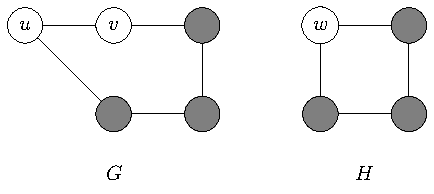
\includegraphics[width=6cm]{bilder/Kantenkontraktion.pdf}
  \caption{Die Kante, die $u$ und $v$ in $G$ verbindet, wird kontrahiert, sodass sie in $H$ durch den neuen Knoten $w$ ersetzt wird.}
  \label{fig:Kantenkontraktion}
\end{wrapfigure}
Die Menge adjazenter Knoten eines Knotens $v$ wird durch $N(v)$ angegeben.
Als \emph{Knotengrad} von $v$ wird die Kardinalität von $N(v)$ bezeichnet.
Bei einer \emph{Kantenkontraktion} einer Kante $e = (u, v)$ wird ein neuer Knoten $w$ hinzugefügt, sodass $N(w) = N(u) \cup N(v)$ gilt und anschließend $e$ aus dem Graphen entfernt.
In \Abb \ref{fig:Kantenkontraktion} ist das Vorgehen skizziert.
Analog kann, wie in \Abb \ref{fig:Pfadkontraktion} gezeigt, ein Pfad kontrahiert werden, indem nacheinander je eine Kante des Pfades kontrahiert wird.
\begin{figure}[H]
  \centering
  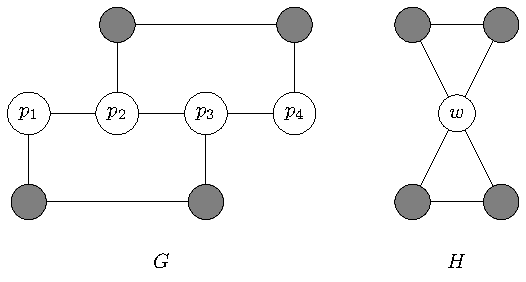
\includegraphics[width=8cm]{bilder/Pfadkontraktion.pdf}
  \caption{Der Pfad von $p_1$ bis $p_4$ wird kontrahiert.
           Der neue Knoten $w$ in $H$ enthält alle Nachbarn der Pfadknoten in $G$.}
  \label{fig:Pfadkontraktion}
\end{figure}

Ein \emph{Minor} $H$ eines Graphen $G$ bezeichnet einen Graph, der isomorph zu $G$ ist, nachdem eine beliebige Menge an Operationen von Kantenkontraktionen, Kantenentfernungen und Knotenentfernungen durchgeführt wurde.
Ein Beispiel dazu findet sich in \Abb \ref{fig:Minor}.
Jeder Graph ist sein eigener Minor, genauso ist jeder Teilgraph ein gültiger Minor.
Dass $H$ ein Minor von $G$ ist, wird dargestellt durch $H$ \minor $G$.
Ist $V$ eine Menge von Knoten, die einen zusammenhängenden Teilgraphen formen, der durch Kontraktionen durch einen neuen Knoten $w$ ersetzt wurde, dann bezeichnet das \emph{Branch-Set} von $w$ die Menge $V$.
In \Abb \ref{fig:Minor} besteht beispielsweise das Branch-Set von $g$ aus $\{a, b, c\}$, zu $f$ in $H_2$ gehört die Knotenmenge $\{f\}$ in $G$.

Für die Knotenmenge $U \subseteq V$ bezeichnet $G - U$ den Teilgraph, der entsteht, wenn alle Knoten aus $U$ mit ihren inzidenten Kanten aus $G$ entfernt werden.
Besteht eine Knotenmenge $\{u\}$ aus nur einem Knoten, wird statt $G - \{u\}$ auch $G - u$ verwendet.
Durch $G(U)$ für $U \subseteq V$ wird der Teilgraph von $G$, dargestellt, der alle Knoten aus $U$ enthält sowie alle Kanten $e = (u, v) \in E$, für die gilt $u, v \in U$.
Für einzelne Knoten $u$ wird statt $G(\{u\})$ vereinfacht $G(u)$ geschrieben.
Eine \emph{Subdivision} $H$ eines Graphen $G$ enthält alle Knoten aus $G = (V, E)$, sodass jedes inzidente Knotenpaar $\{u, v\} \subseteq V$ in $H$ durch einen Pfad verbunden ist.
\begin{figure}[H]
  \centering
  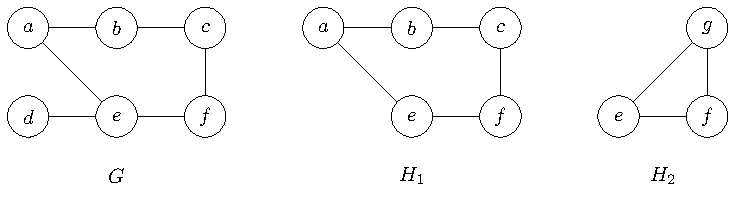
\includegraphics[keepaspectratio]{bilder/Minor.pdf}
  \caption{Ein Graph $G$ mit seinen Minoren $H_1$ und $H_2$.
           Um $H_1$ zu erhalten, wurde in $G$ die Kante $(d, e)$ und anschließend der Knoten $d$ entfernt.
           Für $H_2$ wurden außerdem der Pfad $P(a, c)$ kontrahiert.}
  \label{fig:Minor}
\end{figure}

\begin{wrapfigure}{r}{4cm}
  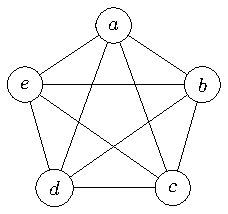
\includegraphics[width=4cm]{bilder/K_5.pdf}
  \caption{Der Graph \kf.}
  \label{fig:K5}
\end{wrapfigure}
Ein Graph wird als \emph{planar} bezeichnet, wenn er sich so in der Ebene einbetten lässt, dass sich keine Kanten kreuzen.
Ein \kf (\sAbb \ref{fig:K5}) ist ein Graph bestehend aus einer Clique von fünf Knoten.
Ein \kdd (\sAbb \ref{fig:K33}) ist ein vollständig bipartiter Graph mit sechs Knoten, sodass jede Bipartition drei Knoten enthält.
Er lässt sich also in zwei Knotenmengen unterteilen (im Folgenden als rote und blaue Menge bezeichnet), sodass alle Knoten der einen Menge zu allen Knoten der anderen Menge benachbart sind.
Nach dem Satz von Kuratowski \cite{Kur30} ist ein Graph genau dann planar, wenn er keine \kf- oder \kdd-Subdivision als Teilgraph beinhaltet.
Eine alternative Formulierung von Wagner \cite{Wag37} sagt aus, dass ein Graph genau dann planar ist, wenn er keinen \kf-Minor oder \kdd-Minor enthält\cite{Die12}.

\ \\
\begin{wrapfigure}{r}{4cm}
  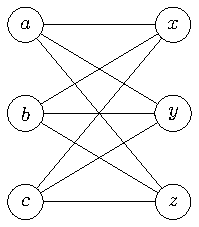
\includegraphics[width=4cm]{bilder/K_33.pdf}
  \caption{Der Graph \kdd.}
  \label{fig:K33}
\end{wrapfigure}
Als nächstes wird ein \kdd genauer betrachtet.
Sei dessen rote Knotenmenge $R = \{a, b, c\}$ und blaue $B = \{x, y, z\}$.
Diese sechs Knoten werden in einer \kdd-Subdivision (analog in einem \kdd-Minor) $H$ \emph{Branch-End} genannt und zeichnen sich dadurch aus, dass sie als einzige Knoten in $H$ den Grad 3 haben.
Ein \emph{Branch-Path} in $H$ ist ein Pfad, der zwei Branch-Ends verbindet, beispielsweise $P(a, x)$.
Ein \emph{Branch-Fan} bezieht sich immer auf eines der Branch-Ends und wird \zB für $a$ als $F(a)$ geschrieben.
Bezeichnet werden dadurch alle Pfade, die zu einem anderen Branch-End führen -- für $a$ also die Pfade $P(a, x)$, $P(a, y)$ und $P(a, z)$.
Zwei Branch-Paths sind \emph{parallel}, wenn ihre Endpunkte vier unterschiedlichen Branch-Ends sind.


Der Graph $W$ bezeichnet einen speziellen Graph, der aus acht Knoten besteht.
Seine äußeren Kanten bilden einen Kreis, außerdem sind die Knoten jeweils adjazent zu den gegenüberliegenden. Eine Darstellung findet sich links in \Abb \ref{fig:W}.
Er enthält einen \kdd als Minor (in der Abbildung rechts angedeutet), jedoch keinen \kf.
Als $M$ wird ein Graph bezeichnet, der einen \kdd als Minor enthält, jedoch einen zusätzlichen Knoten und zwei zusätzliche Kanten hat.
Er ist interessant, weil er, wie in \Abb \ref{fig:M} zu sehen, neben einem \kdd-Minor auch einen \kf-Minor enthält.
\begin{figure}[H]
  \centering
  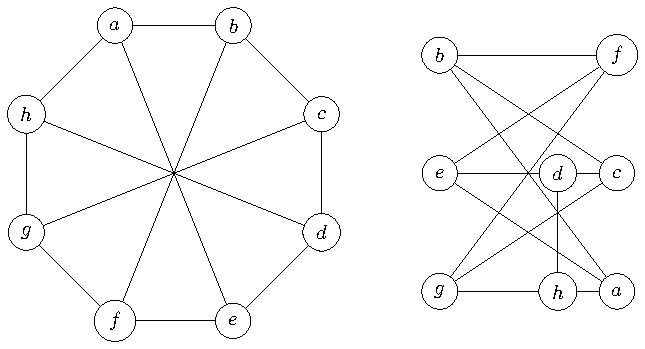
\includegraphics[keepaspectratio]{bilder/W.pdf}
  \caption{Der Graph $W$, links in seiner üblichen Darstellung, rechts mit angedeutetem \kdd-Minor.}
  \label{fig:W}
\end{figure}

\begin{figure}[H]
  \centering
  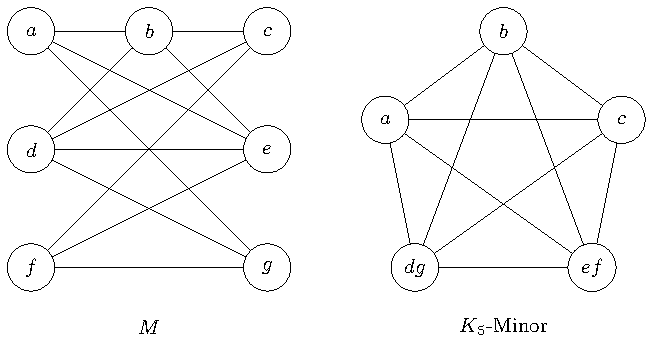
\includegraphics[keepaspectratio]{bilder/M.pdf}
  \caption{Der Graph $M$ sowie ein \kf-Minor aus $M$.}
  \label{fig:M}
\end{figure}

Als \emph{$i$-Separator} wird eine Menge $S$ bestehend aus $i$ Knoten in einem zusammenhängenden Graphen $G$ bezeichnet, sodass $G - S$ nicht mehr zusammenhängend ist.
Ein Graph ist \emph{$k$-zusammenhängend}, falls er keinen $(k-1)$-Separator enthält.
Ein \emph{$(i, j)$-Separator} ist ein $i$-Separator, sodass $G-S$ aus mindestens $j$ Zusammenhangskomponenten besteht.
In \Abb \ref{fig:AugmentierteKomponenten} wird ein \dd-Separator im oberen Graphen gezeigt, der aus den Knoten $\{c_1, c_2, c_3\}$ besteht.
Sind $C \subset V$ die $i$ Knoten, die zu einem $(i, j)$-Separator in $G$ gehören, wird der Graph durch $G - C$ zunächst in $j$ Zusammenhangskomponenten $Z_1, ..., Z_j$ zerlegt.
Dann wird für jedes $Z_k$ mit $1 \leq k \leq j$ ein neuer Graph $A_k$ erzeugt, der aus dem Teilgraphen $Z_k \cup C$ besteht -- die Knoten von $C$ in $A_k$ werden paarweise durch Kanten verbunden, falls sie noch nicht adjazent zueinander sind.
Jeder der resultierenden Graphen wird als \emph{augmentierte Komponente} des Eingabegraphen $G$ bezeichnet, die durch den Separator $C$ definiert wird.

Ist $V$ eine Menge von Knoten oder Kanten, dann bezeichnet $\vert V \vert$ die Kardinalität von $V$.
Sei $A_1$ ein Graph mit einer Clique $C_1$ und $A_2$ ein Graph mit einer Clique $C_2$, sodass $\vert C_1 \vert = \vert C_2 \vert = i$ ist.
Dann bezeichnet eine Cliquen-Summe das paarweise Zusammenfügen von je einem Knoten $c_1 \in C_1$ mit einem $c_2 \in C_2$, sodass ein neuer Graph $G$ entsteht, der sowohl einen $A_1$-, als auch einen $A_2$-Minor enthält.
Innerhalb einer solchen Operation dürfen zusätzlich beliebige Kanten in $G$ gelöscht werden, die zwei Knoten in der Clique verbinden.
Dadurch ist es möglich, einen Graphen $G$ durch einen Separator in augmentierte Komponente aufzuteilen und anschließend durch eine Cliquen-Summe wieder $G$ zu erhalten.
Dieses Vorgehen wird in \Abb \ref{fig:AugmentierteKomponenten} gezeigt, dabei wird der obere Graph in die unten abgebildeten augmentierten Komponenten aufgeteilt \bzw von unten nach oben werden drei Graphen durch eine Cliquen-Summe zusammengefügt.
\begin{figure}[H]
  \centering
  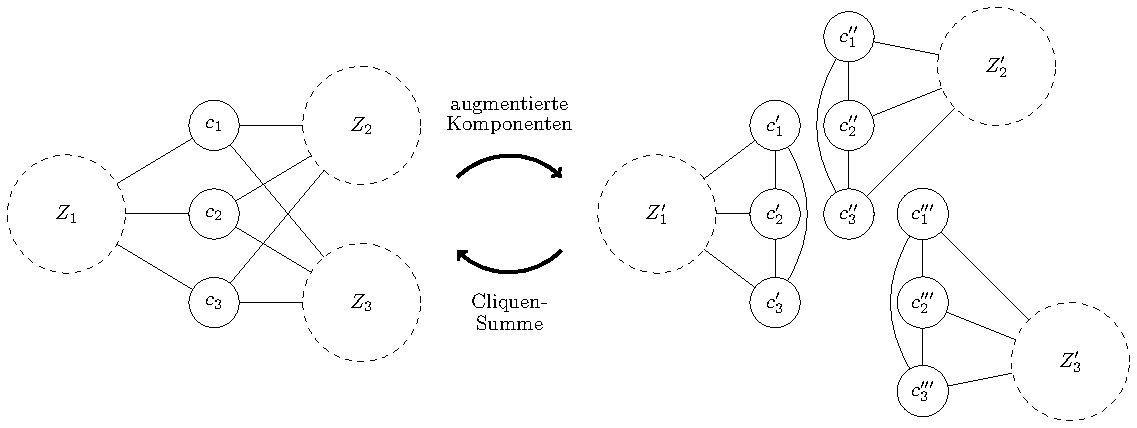
\includegraphics[keepaspectratio]{bilder/Augmentierte_Komponenten.pdf}
  \caption{Der obere Graph wird in drei augmentierte Komponenten durch den \dd-Separator $C = \{c_1, c_2, c_3\}$ geteilt.
           Alle $Z_i$ und $Z_i'$ stellen Teilgraphen dar, die zur Übersicht zu einem Knoten zusammengefügt wurden.
           Aus den drei unteren Graphen kann durch die Cliquen-Summe der Cliquen $\{c_1', c_2', c_3'\}$ sowie $\{c_1'', c_2'', c_3''\}$ und $\{c_1''', c_2''', c_3'''\}$ der oberen Graphen erzeugt werden.
           Während der Cliquen-Summen Operation dürfen beliebige Kanten, die die Knoten in den Cliquen verbinden, gelöscht werden.}
  \label{fig:AugmentierteKomponenten}
\end{figure}
